% ============================================================
% Section 1: Introduction & Intuition
% ============================================================
\section{Introduction \& Intuition}

\begin{frame}{Historical Context}
    The paper about Mean Shift was first introduced by \textbf{Fukunaga and Hostetler in 1975} with the 
    title \textit{"The Estimation of the Gradient of a Density Function, with Applications in Pattern Recognition"}
    where they presented the mean shift algorithm as a method for finding modes of a density function given discrete data sampled from that function.

    \vspace{0.5cm}

    Later on in 2002, \textbf{Comaniciu and Meer} popularized the algorithm in their paper 
    \textit{"Mean Shift: A Robust Approach Toward Feature Space Analysis"} by demonstrating
    its effectiveness in computer vision tasks such as image segmentation and tracking.
\end{frame}

\begin{frame}{What is Mean Shift Clustering?}
    \begin{columns}[T]
        \begin{column}{0.5\textwidth}
            \textbf{Core Idea:}
            \begin{itemize}
                \item Find modes (peaks) of data density
                \item Points converge to nearest mode
                \item No need to specify number of clusters
                \item Density-based approach
            \end{itemize}

            \vspace{0.5cm}

            \textbf{Key Characteristic:}
            \begin{itemize}
                \item \textcolor{customred}{Non-parametric}
                \item Discovers clusters naturally
                \item Based on kernel density estimation
            \end{itemize}
        \end{column}

        \begin{column}{0.5\textwidth}
            \begin{center}
                \begin{tikzpicture}[scale=0.8]
                    % Draw density surface (simplified)
                    \draw[thick, customred] plot[smooth, tension=0.7] coordinates {
                        (0,1) (1,1.5) (2,3) (3,1.5) (4,1) (5,2.5) (6,1)
                    };

                    % Draw points
                    \foreach \x in {1.8,2,2.2,5,5.2} {
                        \fill (\x,0.2) circle (2pt);
                    }

                    % Draw arrows showing convergence
                    \draw[->, thick, blue] (1.8,0.2) -- (2,2.5);
                    \draw[->, thick, blue] (2.2,0.2) -- (2,2.5);
                    \draw[->, thick, blue] (5,0.2) -- (5.1,2);

                    % Label modes
                    \node[customred] at (2,3.3) {Mode 1};
                    \node[customred] at (5,2.8) {Mode 2};

                    % Axes
                    \draw[->] (0,0) -- (6.5,0) node[right] {$x$};
                    \draw[->] (0,0) -- (0,3.5) node[above] {Density};
                \end{tikzpicture}
            \end{center}
            \small{\textit{Points shift toward density peaks}}
        \end{column}
    \end{columns}
\end{frame}

\begin{frame}{Visual Intuition}
    \textbf{Think of it as:}
    \begin{enumerate}
        \item Imagine data points as balls on a hilly landscape
        \item Each ball rolls uphill to the nearest peak
        \item Balls ending at the same peak = same cluster
    \end{enumerate}

    \vspace{0.5cm}

    \begin{center}
        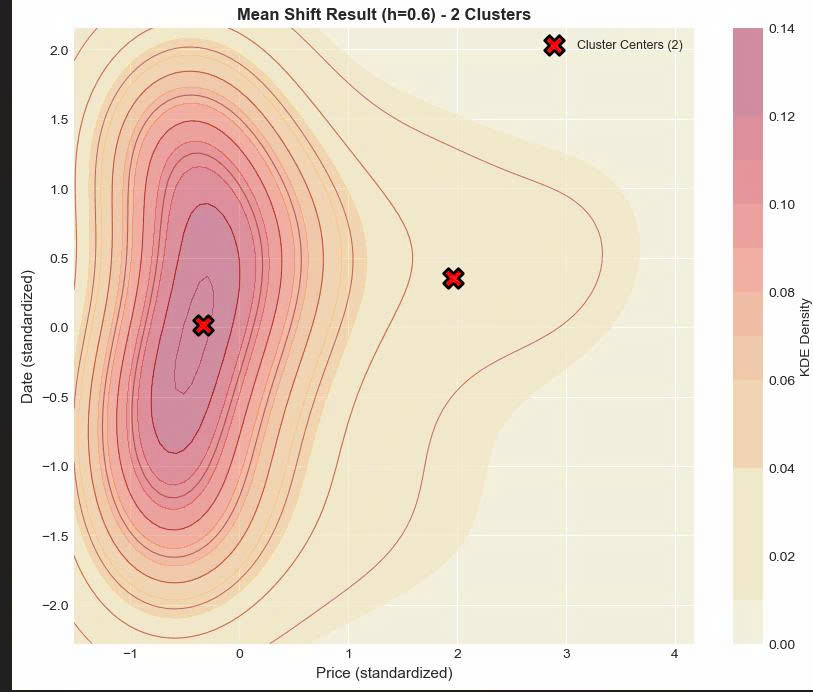
\includegraphics[width=0.3\textwidth]{images/image.png}
    \end{center}

    \textbf{Advantage:} Discovers cluster count automatically from data!
\end{frame}
